\documentclass[10pt]{article}
\usepackage[utf8]{inputenc}
\usepackage[T1]{fontenc}
\usepackage{amsmath}
\usepackage{amsfonts}
\usepackage{amssymb}
\usepackage[version=4]{mhchem}
\usepackage{stmaryrd}
\usepackage{hyperref}
\usepackage{graphicx}
\graphicspath{ {./CS-234/} }

\title{Assignment 1 - Sets }

\author{CS 234}
\date{Daniel Lee}


\begin{document}
\maketitle

\section*{1 \quad Part A - Sets on Paper}

\begin{enumerate}
      \item [1.3] Write out the elements of the following sets within set braces:


            $\{2 n: n \in \mathbb{N}, n<5\}$
            \\ $\{0, 2, 4, 6, 8\}$

      \item [1.14] Write the following sets using set-builder notation:

            $\{0, 1, 4, 9, 16,...$\}
            \\ $\{n^2: n \in \mathbb{N}\}$

      \item [1.19 \& 1.23] Assuming that $A=\{1,2,3,4,5\}, B=\{2,3,5,7\}, C=\{4,5,6,7,8\}$ and a universal set $U=\{1,2,3,4,5,6,7,8\}$, compute the following:


            1.19. B $-$ C = $\{2, 3\}$
            \\
            \\ 1.23. $(A \cup B) \cap(\overline{B \cup C})=\{1\}$

      \item [1.28] Draw Venn diagrams for the following expressions, showing the steps (intermediate diagrams) in each case:

            $\bar{A} \cap \bar{B} \cap \bar{C}$


            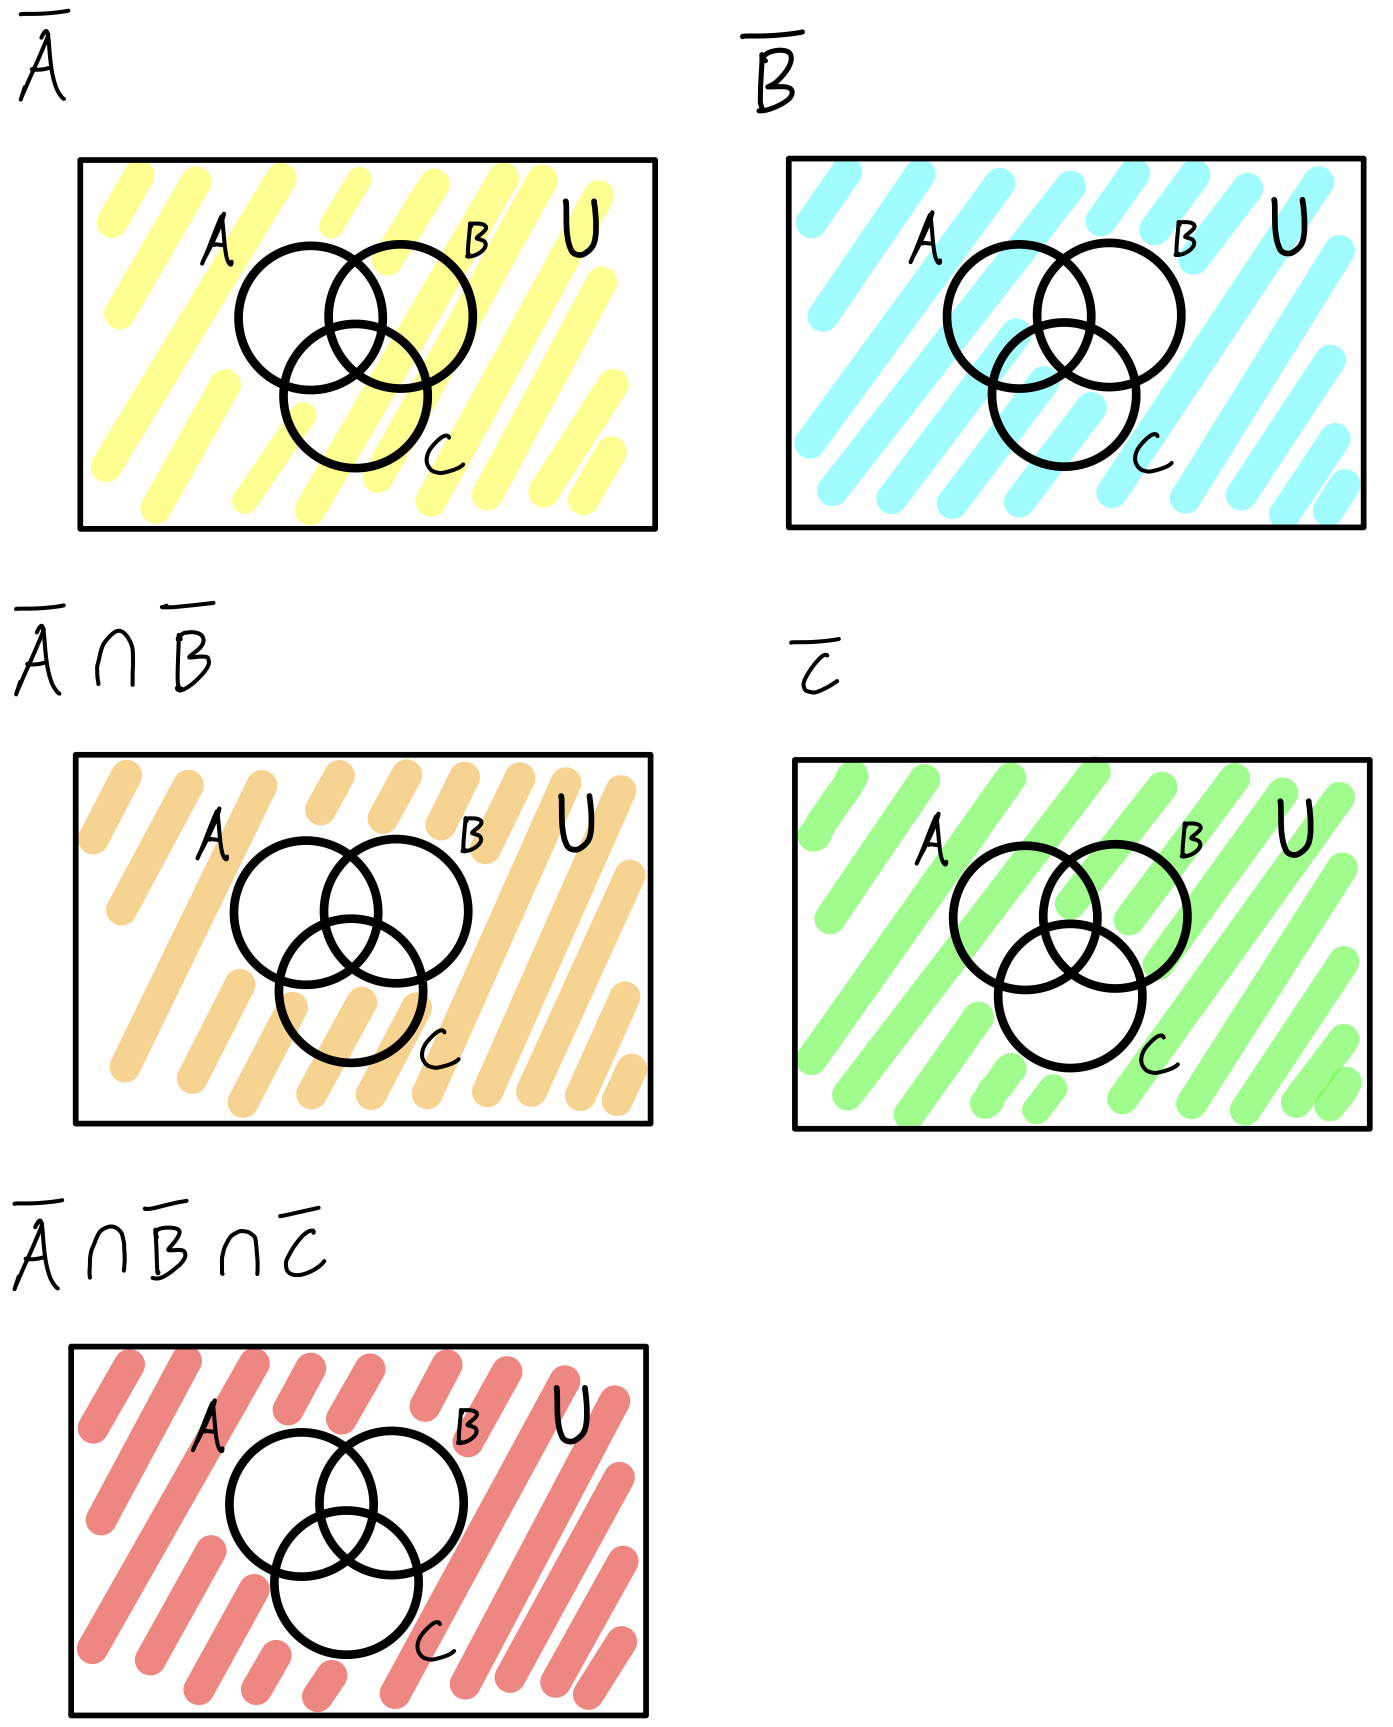
\includegraphics[scale=0.2]{venn1}

      \item [1.32] Show using Venn diagrams, using labeled intermediate steps, whether the following pairs of expressions are equal:

            $C-(A \cup B)$ and $(C-A) \cap(C-B)$


            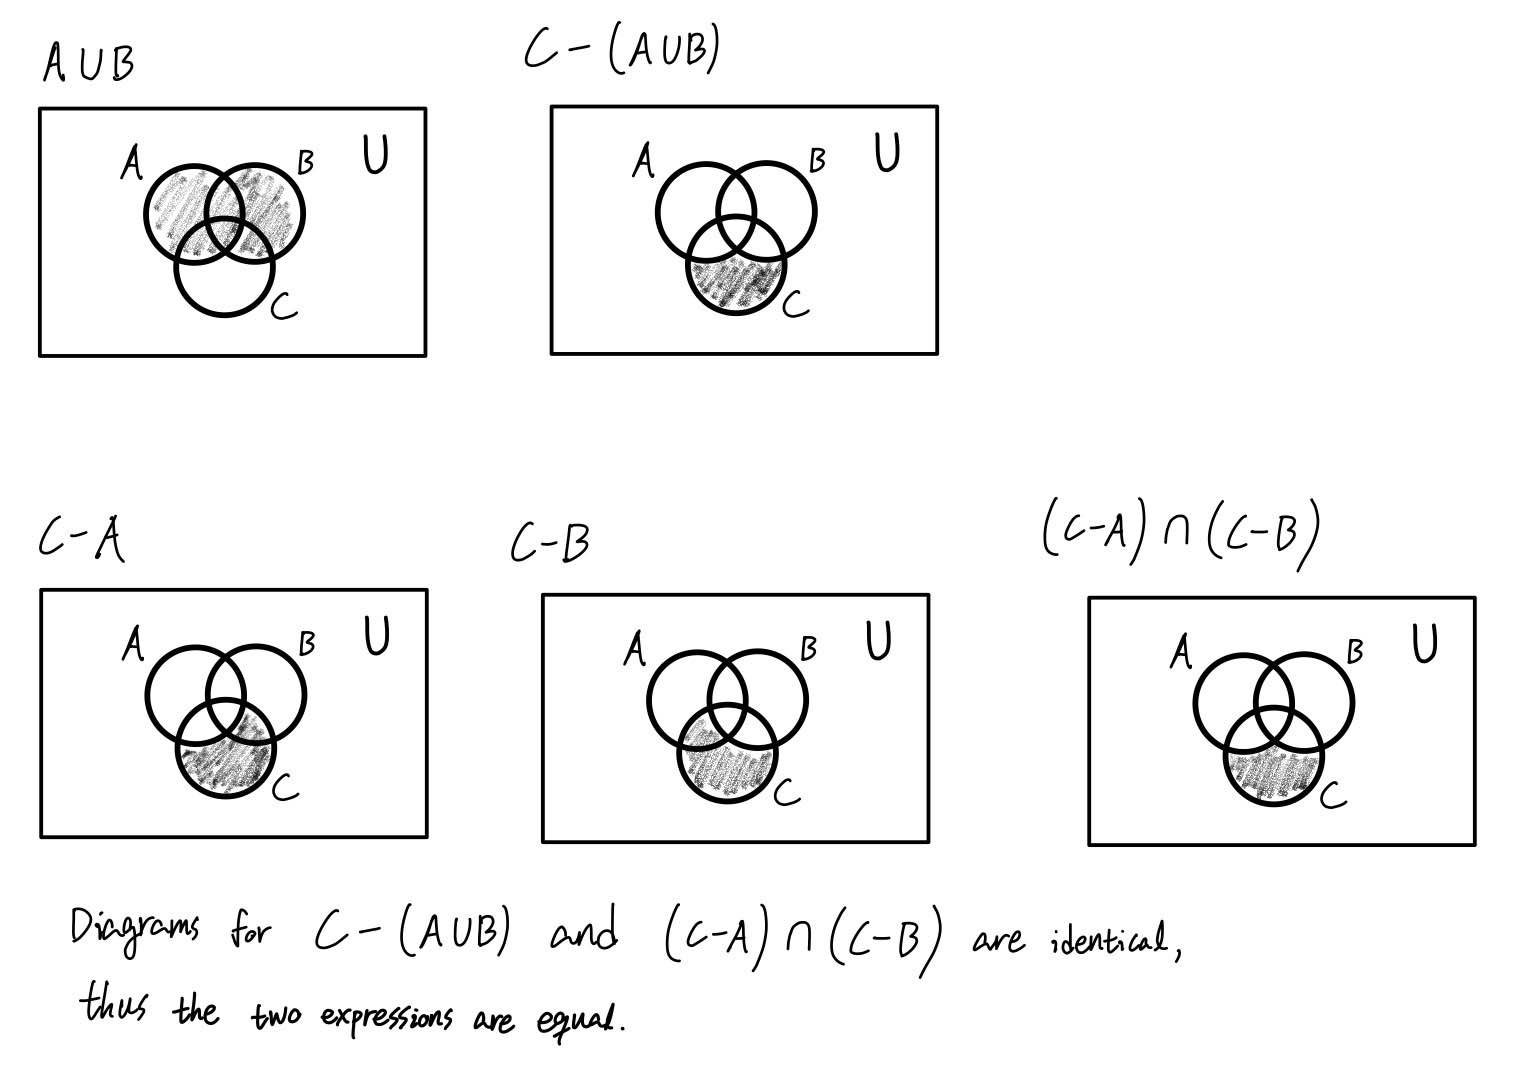
\includegraphics[scale=0.18]{venn2}

      \item [1.36] List the elements of the following sets within set braces:

            $\mathcal{P}(\{a,\{b, c\}\})$

            $\{\emptyset , \{a\}, \{\{b, c\}\}, \{a, \{b, c\}\}\}$

      \item [1.44] Compute the size of each of the following sets:

            $\mathcal{P}(\mathcal{P}(\mathcal{P}(\{0,1\})))$

            $2^{16} = 65536$

      \item [1.47 \& 1.52] Assuming that $A=\{0,1\}, B=\{a, b\}$ and $C=\{1,2,3\}$, list the elements of the following sets within set braces:

            1.47. $C^2$
            \\$\{(1,1), (1,2), (1,3), (2,1), (2,2), (2,3), (3,1), (3,2), (3,3)$\}


                  1.52. $A \times(B \times C)$
            \\$\{(0,(a,1)), (0,(a,2)), (0,(a,3)), (0,(b,1)), (0,(b,2)), (0,(b,3)), (1,(a,1)), (1,(a,2)), (1,(a,3)),
            \\(1,(b,1)), (1,(b,2)), (1,(b,3))\}$

      \item [1.58] Assuming that $A=\{0,1\}, B=\{a, b\}$ and $C=\{1,2,3\}$, compute the size of each of the following sets:

            $\mathcal{P}(\mathcal{P}(A) \times \mathcal{P}(B) \times \mathcal{P}(C)) = 2^{128}$

      \item [1.61 \& 1.62] List the domain and the codomains for the following functions:

            1.61. A function sum that takes as input 10 real numbers and returns their sum.

            Domain: $\mathbb{R}^{10}$

            Codmoain: $\mathbb{R}$


            1.62. A function sort5 that takes as input 5 integers and returns them sorted.

            Domain: $\mathbb{Z}^{5}$

            Codmoain: $\mathbb{Z}^{5}$

      \item [1.66] Write out the following strings in shorthand notation:

            abcabcabcabc
            \\$(abc)^4$

      \item [1.71] Write out all the prefixes and suffixes for the following strings:

            aaabbccc
            \\ Prefixes: $\lambda$, a, aa, aaa, aaab, aaabb, aaabbc, aaabbcc, aaabbccc
            \\ Suffixes: $\lambda$, c, cc, ccc, bccc, bbccc, abbccc, aabbccc, aaabbccc

      \item [1.78] List all strings of length at most 4 from the following languages:

            $\Sigma = \{0, 1\}$
            \\
            \\$\left\{x 11 y: x, y \in \Sigma^*\right\}$

            11, 011, 110, 111, 1110, 0111, 1111, 0011, 1100, 1101, 1011, 0110

      \item [1.88 \& 1.90] Write the following languages in set builder (mathematical) notation:

            $\Sigma = \{a, b\}$
            \\
            \\1.88. The set of all strings that have an even number of as followed by an odd number of bs.

            $\{a^{2n}b^{2m+1} : n,m\in \mathbb{N} \}$


            1.90. The set of all strings that have an a in the third position.

            $\{xyaz : x, y \in \{a, b\}$ and $z \in \{a,b\}^{*} \}$


      \item [A.1] Multiplication rule (repeats allowed, order matters)

            How many license plates are possible with a three letter combination followed by a 4 digit number? (Note: the number may have a leading 0.)

            $$26^3 \times 10^4 = 175760000$$

      \item [A.9] Permutations (no repeats, order matters)

            You’re going on a road trip with seven other friends and have room for three of them in your car. If it matters which seat each person takes (front passenger’s seat, rear left, and rear right), then how many ways are there to pick friends for your car?

            $$7 \times 6 \times 5 = 210$$

      \item [A.11] Basic combinations (no repeats, order doesn’t matter)

            How many ways are there to select a four person group from a class of 20 students?

            $$\binom{20}{4}=\frac{20!}{16!4!}=\frac{20 \times 19 \times 18 \times 17}{1 \times 2 \times 3 \times 4}=4845$$


\end{enumerate}

\end{document}